\chapter{Subjective Timbre Evaluation}
\label{chap:ListeningTests}
	\todo{Come up with a better name for this chapter.}

\section{Production Environment Timbre Evaluation} % this name will probably change
\label{sec:ListeningTests-DAWBasedTimbreEvaluation}
The perceptual listening test methodologies discussed in Section \ref{sec:Timbre-ListeningTests} rely on the participants
performing a certain set of tasks. While this structure helps to reduce the number of variables in an experiment it does not
necessarily reflect the way audio is treated in a production environment.

A new methodology has been developed in which the analysis of timbre is introduced into a typical music production workflow
causing minimal interruption to the producer. This methodology aims to answer the question "What terms do music producers
use to describe the timbral transformations they apply to audio during the creation of music?". 

This section will detail what the typical production workflow is and how semantic information can be gathered.

	\subsection{Music Production Workflow}
		\todo{Find some references for this section. Probably mixing engineers handbook or something.}

		The music production workflow has four main stages:

		\begin{itemize}
			\item Recording
			\item Editing
			\item Mixing
			\item Mastering
		\end{itemize}

		At every stage of this process semantic descriptors are often used to communicate the desired timbral
		qualities of the audio. For instance one my ask that a certain microphone be used because of the `warmth' it
		adds to the recorded sound. During the mixing and mastering stages audio processing effects are applied to
		shape the timbre further.  These stages will be the focus of this section as the aim of this thesis is to
		improve the intuitiveness of these effects.

		Historically audio effects were pieces of electronic hardware through which an audio signal is passed.
		Modern music production techniques utilise Digital Audio Workstation (DAW) software. This software enables
		users to record, edit and mix multiple tracks of audio using a computer. 
		
	\subsection{Analysis of Timbre Inside the DAW}
		An ideal way to collect timbral information during music production would be to have the DAW analyse the
		audio tracks used and production techniques applied. Information which could be gathered directly from the
		DAW, with no extra input from the user, includes:

		\begin{itemize}
			\item Information about the audio processing chain:
			\begin{itemize}
				\item The effects applied to each track.
				\item The order in which these effects are applied.
				\item The parameter settings of these effects.
			\end{itemize}

			\item Features of the audio signal at every stage in the processing chain.
		\end{itemize}

		Additional information can be gathered by prompting the user for input:

		\begin{itemize}
			\item The genre of music being produced.
			\item The content of the separate audio tracks (what instruments etc.).
			\item Semantic terms which describe the timbral transformations applied by each audio
			      effect.
		\end{itemize}

		Achieving this would require the creation of a new DAW. This would be impractical for the current research.
		DAWs are very comprehensive software packages which perform many more tasks than the application of effects
		to audio (project management, audio editing functionality etc.). A lot of effort would be expended in
		implementing these features before any timbral data could be collected.  Music producers also tend to have a
		preferred DAW with which they work most fluidly. Convincing producers to use a new DAW, for the purposes of
		research, would be a difficult task.

		Third party developers can produce extensions to DAWs known as plug-ins. Plug-Ins provide additional audio
		processing functionality to the DAW environment. They can optionally expose their own parameters which users
		can adjust to achieve their desired effect. There are several different formats in which audio plug-ins can
		be distributed (VST, AU etc.). Most of the commonly used DAWs support plug-ins in one or more of these
		formats.

		Audio plug-ins provide a good platform to allow producers to provide semantic terms and audio feature
		information from within their preferred DAW. As part of this research a suite of audio plug-ins which
		extract this information have been developed. They have been release under the title Semantic Audio Feature
		Extraction (SAFE) Plug-Ins.

	\subsection{SAFE Plug-Ins}
		The SAFE plug-ins consist of four commonly used audio effects: Equaliser, Distortion, Compressor and Reverb.
		As part of the plug-ins's interface the user has the option to save semantic terms. The interface for the
		SAFE Distortion is shown in Figure \ref{fig:SAFE-Distortion}. Upon saving terms the plug-in will analyse the
		audio at its inputs and outputs. When the analysis is completed the results are stored, containing:

		\begin{itemize}
			\item The users description of the timbre.
			\item The plug-in's current parameter settings.
			\item The features of the audio before and after processing.
			\item Some additional data about the user and the track being worked on.
			\begin{itemize}
				\item The genre.
				\item The instrument.
				\item The users age.
				\item The users location.
				\item The users primary language.
				\item The number of year experience the user has in music production.
			\end{itemize}
		\end{itemize}

		\begin{figure}[h!]
			\centering
			\includegraphics[width=0.8\textwidth]{chapter4/Images/SAFEDistortion.png}
			\caption{The Interface for the SAFE Distortion Plug-In}
			\label{fig:SAFE-Distortion}
		\end{figure}

		The LibXtract library \citep{bullock2007libxtract} is used in the analysis of the audio. Every scalar
		feature available within LibXtract is calculated along with the MFCCs and Bark Band Coefficients. In total
		five seconds of audio is analysed in frames of 4096 samples each.

		\note{Why 4096 samples? The real reason is because LibXtract works better that way. Will that cut the
		mustard?}

		One disadvantage in using plug-ins is that they cannot gather information about the processing chain they
		may be a part of. The timbral transformation the user is describing may be the result of several effects
		working together. This can be mitigated somewhat by asking users to describe only the effect the plug-in in
		question is providing.

		The SAFE plug-ins also suffer from the same issues other distributed tests do. The researcher forfeits
		control over the listening environment in order to gather results from a much larger sample of people. In
		fact they provide even lest control that methodologies like that used in the Social EQ project
		\citep{cartwright2013socialeq} in that the choice of audio samples being used is decided by the test
		subject. 

\section{Analysis}
\label{sec:ListeningTests-Analysis}

	\begin{figure}[h!]
		\centering
		\subfloat[Individual Transforms]
		{
			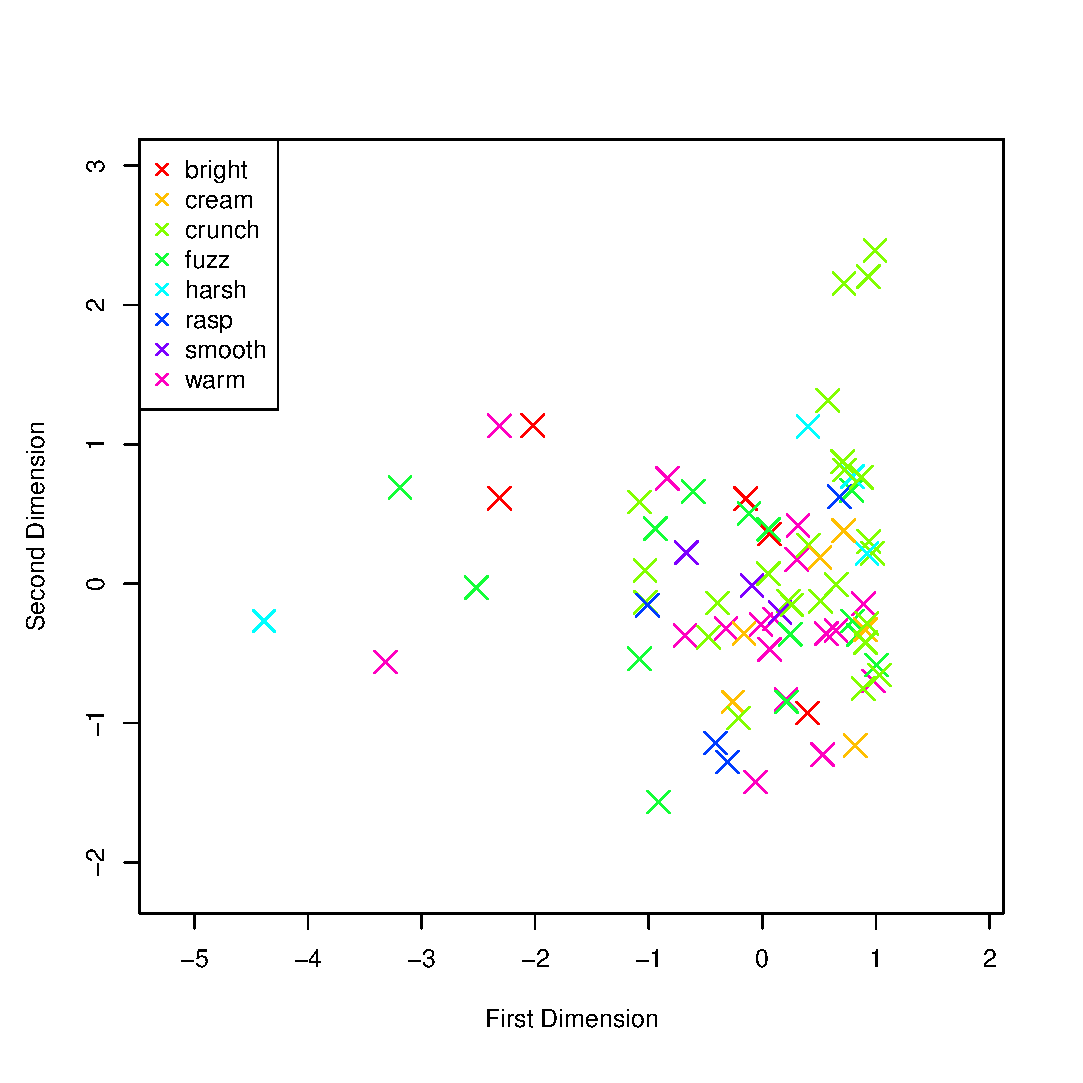
\includegraphics[width=0.45\textwidth]{chapter4/Images/DistortionProcessedMDS.eps}
			\label{fig:DistortionProcessedMDS}
		}
		\qquad
		\subfloat[Descriptor Centroids]
		{
			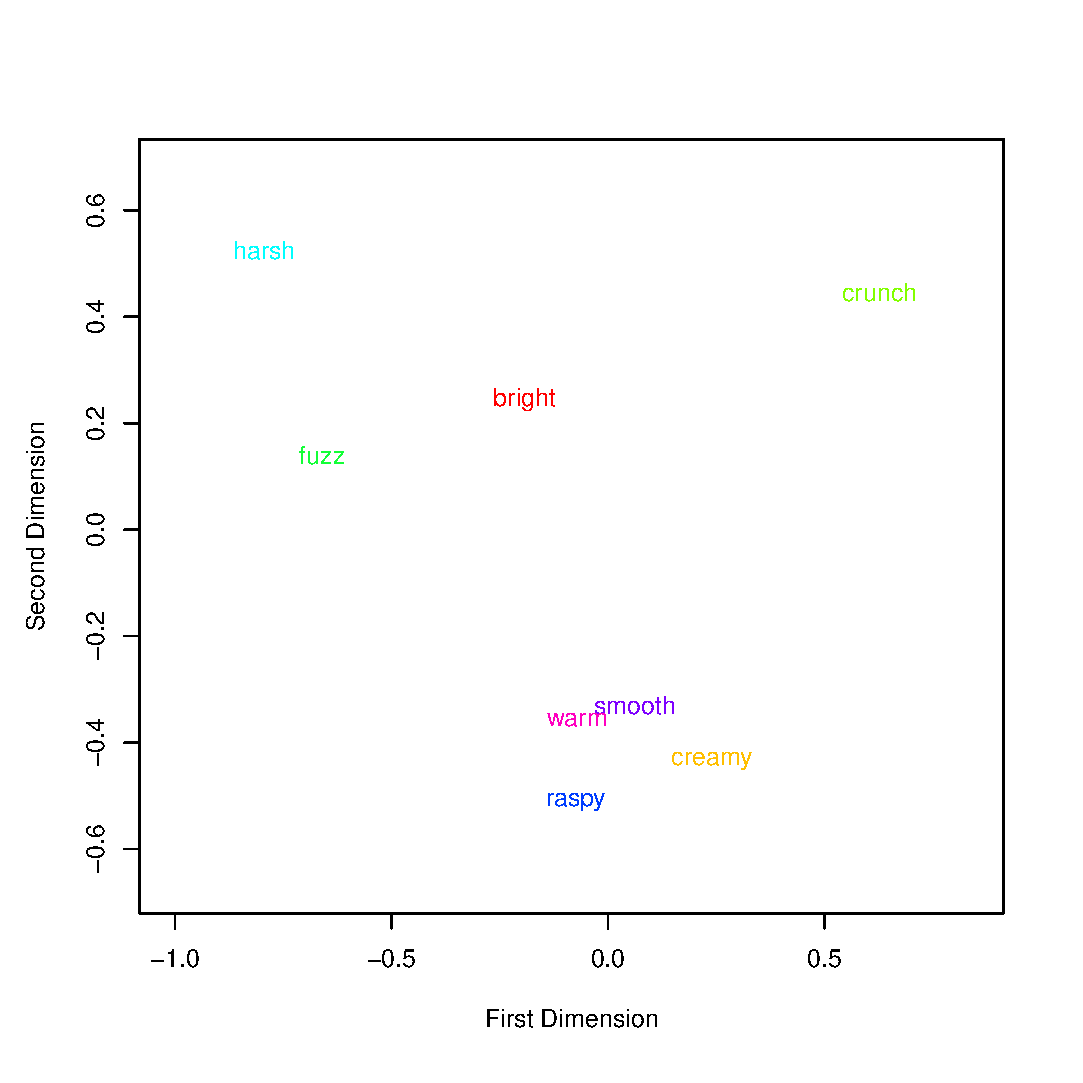
\includegraphics[width=0.45\textwidth]{chapter4/Images/DistortionProcessedCentroidsMDS.eps}
			\label{fig:DistortionProcessedCentroidsMDS}
		}
		\caption{Timbre Space for the Processed Features form the Distortion.}
		\label{fig:DistortionProcessedMDSs}
	\end{figure}

	\begin{table}[h!]
		\centering
		\begin{tabular}{|c|c|c|}
			\hline
			\bf{Feature} & \bf{Correlation} & \bf{p-value} \\
			\hline
			\hline
			Irregularity K & -0.981702638254498 & 5.86525860866353e-37 \\
			\hline
			Peak Irregularity K & -0.962036042628834 & 2.73321934750131e-29 \\
			\hline
			Bark Coefficient 6 & -0.959036054870656 & 1.70190172876899e-28 \\
			\hline
			Peak Spectral Kurtosis & -0.940033366324044 & 1.55053342301828e-24 \\
			\hline
			Bark Coefficient 7 & -0.936553028504178 & 5.93192971807379e-24 \\
			\hline
			Harmonic Irregularity K & -0.933019146143437 & 2.14810473054194e-23 \\
			\hline
			Harmonic Spectral Kurtosis & -0.924326438294474 & 3.85764808897598e-22 \\
			\hline
			Bark Coefficient 5 & -0.922957072163232 & 5.89092885576859e-22 \\
			\hline
			Peak Spectral Skewness & -0.920984402717623 & 1.06945158126544e-21 \\
			\hline
			Bark Coefficient 8 & -0.914782358316355 & 6.33230467348598e-21 \\
			\hline
		\end{tabular}
		\caption{Significant Features for Dimension 1 of the Timbre Spaces Shown in Figure 
			 \ref{fig:DistortionProcessedMDSs}.}
		\label{tab:DistortionProcessedFeaturesDim1}
	\end{table}

	\begin{table}[h!]
		\centering
		\begin{tabular}{|c|c|c|}
			\hline
			\bf{Feature} & \bf{Correlation} & \bf{p-value} \\
			\hline
			\hline
			Spectral Centroid & 0.934357264112107 & 0 \\
			\hline
			Spectral Roll Off & 0.920245205497915 & 0 \\
			\hline
			MFCC 1 & -0.896491813212876 & 5.98001677533564e-19 \\
			\hline
			Spectral Slope & 0.883921167187462 & 0 \\
			\hline
			Peak Spectral Standard Deviation & 0.85800083369724 & 8.88178419700125e-16 \\
			\hline
			Harmonic Spectral Standard Deviation & 0.856326749640604 & 1.11022302462516e-15 \\
			\hline
			Harmonic Spectral Centroid & 0.847853863903556 & 4.21884749357559e-15 \\
			\hline
			Peak Spectral Centroid & 0.846379278425876 & 5.10702591327572e-15 \\
			\hline
		\end{tabular}
		\caption{Significant Features for Dimension 2 of the Timbre Spaces Shown in Figure 
			 \ref{fig:DistortionProcessedMDSs}.}
		\label{tab:DistortionProcessedFeaturesDim2}
	\end{table}

	\begin{figure}[h!]
		\centering
		\subfloat[Individual Transforms]
		{
			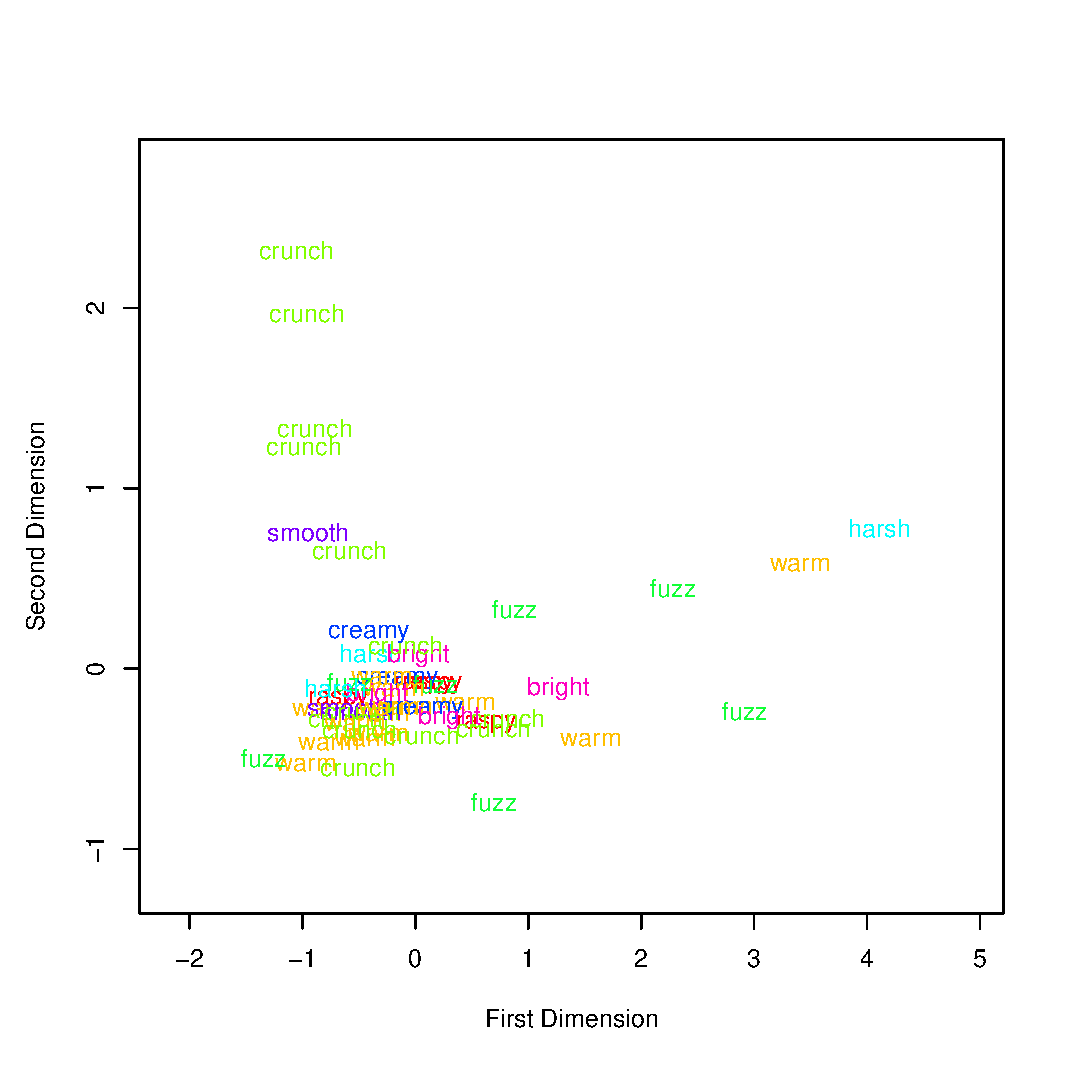
\includegraphics[width=0.45\textwidth]{chapter4/Images/DistortionDifferenceMDS.eps}
			\label{fig:DistortionDifferenceMDS}
		}
		\qquad
		\subfloat[Descriptor Centroids]
		{
			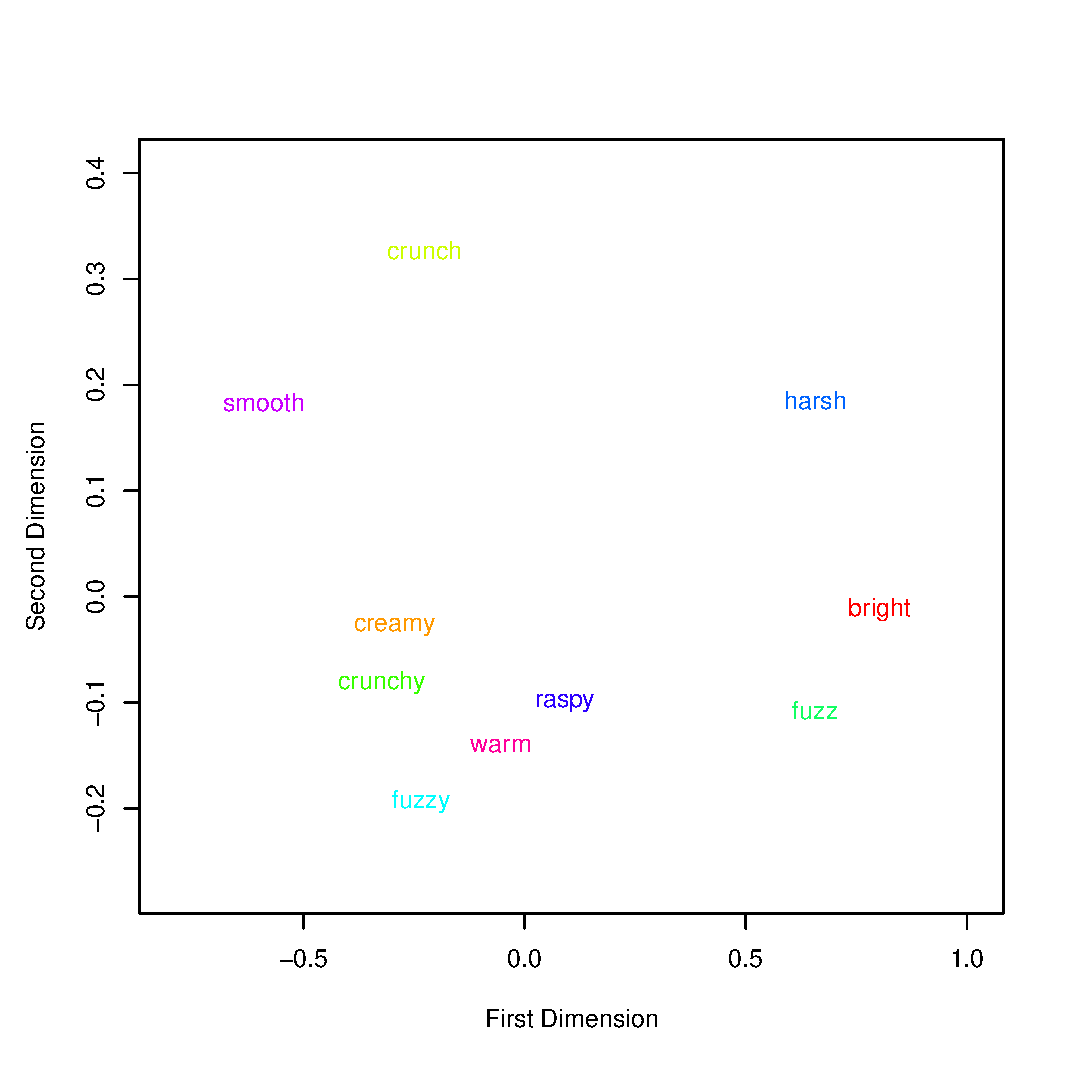
\includegraphics[width=0.45\textwidth]{chapter4/Images/DistortionDifferenceCentroidsMDS.eps}
			\label{fig:DistortionDifferenceCentroidsMDS}
		}
		\caption{Timbre Space for the Feature Differences form the Distortion.}
		\label{fig:DistortionDifferenceMDSs}
	\end{figure}

	\begin{table}[h!]
		\centering
		\begin{tabular}{|c|c|c|}
			\hline
			\bf{Feature} & \bf{Correlation} & \bf{p-value} \\
			\hline
			\hline
			Irregularity K & -0.985498074073924 & 2.05802067103551e-39 \\
			\hline
			Peak Irregularity K & -0.965585436473341 & 2.57014502660263e-30 \\
			\hline
			Bark Coefficient 6 & -0.95894018547053 & 1.8002297365022e-28 \\
			\hline
			Bark Coefficient 7 & -0.957021574844167 & 5.39083077911368e-28 \\
			\hline
			Bark Coefficient 15 & -0.952417240055253 & 6.18694971512614e-27 \\
			\hline
			Bark Coefficient 8 & -0.951360019811739 & 1.04712187507916e-26 \\
			\hline
			Bark Coefficient 9 & -0.951137188781872 & 1.16818996425268e-26 \\
			\hline
			Harmonic Irregularity K & -0.949155160917441 & 3.02442464624862e-26 \\
			\hline
			Bark Coefficient 10 & -0.937968421097708 & 3.46968829494617e-24 \\
			\hline
			Bark Coefficient 5 & -0.934441590399684 & 1.29078670910454e-23 \\
			\hline
		\end{tabular}
		\caption{Significant Features for Dimension 1 of the Timbre Spaces Shown in Figure 
			 \ref{fig:DistortionDifferenceMDSs}.}
		\label{tab:DistortionDifferenceFeatures}
	\end{table}

	\begin{table}[h!]
		\centering
		\begin{tabular}{|c|c|c|}
			\hline
			\bf{Feature} & \bf{Correlation} & \bf{p-value} \\
			\hline
			\hline
			Spectral Variance & -0.875525916695384 & 4.27315930700177e-17 \\
			\hline
			Spectral Roll Off & -0.8728405861589 & 6.98033103314871e-17 \\
			\hline
			Harmonic Spectral Centroid & -0.868256190058225 & 1.57333943755696e-16 \\
			\hline
			Harmonic Spectral Standard Deviation & -0.865564070871415 & 2.50031776893959e-16 \\
			\hline
			Peak Spectral Centroid & -0.850640310222172 & 2.752907039677e-15 \\
			\hline
			Spectral Centroid & -0.843402134079256 & 8.0379337150603e-15 \\
			\hline
			Peak Spectral Standard Deviation & -0.822865543302491 & 1.28007959107212e-13 \\
			\hline
			Peak Spectral Variance & -0.817293786410897 & 2.55259503107424e-13 \\
			\hline
			Harmonic Spectral Variance & -0.812345974117126 & 4.62139755362114e-13 \\
			\hline
		\end{tabular}
		\caption{Significant Features for Dimension 2 of the Timbre Spaces Shown in Figure 
			 \ref{fig:DistortionDifferenceMDSs}.}
		\label{tab:DistortionDifferenceFeatures}
	\end{table}

	\begin{figure}[h!]
		\centering
		\subfloat[Individual Transforms]
		{
			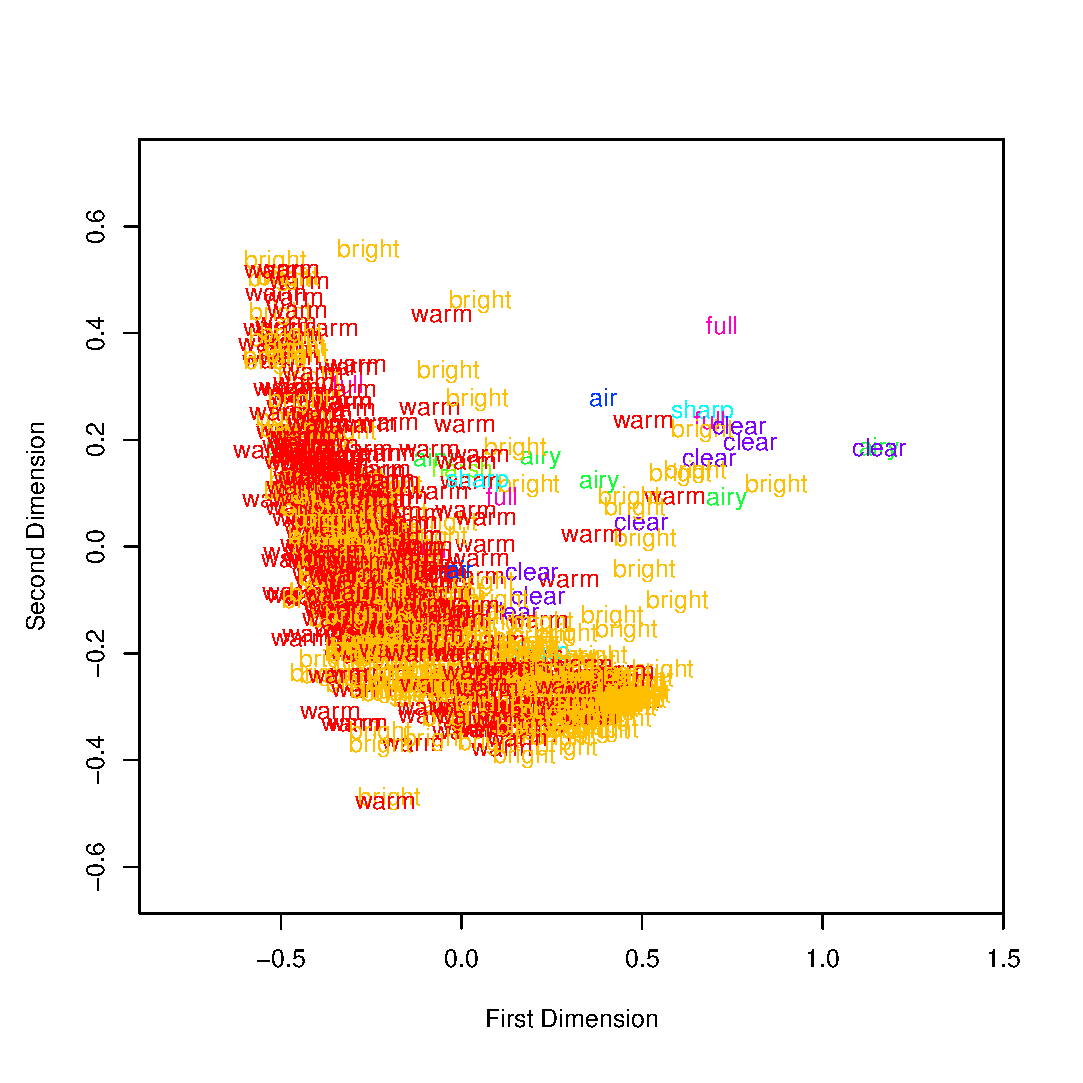
\includegraphics[width=0.45\textwidth]{chapter4/Images/EqualiserProcessedMDS.eps}
			\label{fig:EqualiserProcessedMDS}
		}
		\qquad
		\subfloat[Descriptor Centroids]
		{
			\includegraphics[width=0.45\textwidth]{chapter4/Images/EqualiserProcessedCentroidsMDS.eps}
			\label{fig:EqualiserProcessedCentroidsMDS}
		}
		\caption{Timbre Space for the Processed Features form the Equaliser.}
		\label{fig:EqualiserProcessedMDSs}
	\end{figure}

	\begin{table}[h!]
		\centering
		\begin{tabular}{|c|c|c|}
			\hline
			\bf{Feature} & \bf{Correlation} & \bf{p-value} \\
			\hline
			\hline
			Peak Tristimulus 2 & 0.855583627112928 & 0 \\
			\hline
			Spectral Crest & 0.846391686145526 & 0 \\
			\hline
			Harmonic Tristimulus 2 & 0.843557935487663 & 0 \\
			\hline
			Harmonic Spectral Standard Deviation & -0.827375175520425 & 1.94505570441165e-223 \\
			\hline
			Peak Spectral Standard Deviation & -0.82480168108147 & 7.20182231471735e-221 \\
			\hline
			Bark Coefficient 17 & -0.812395528135387 & 4.72470887847481e-209 \\
			\hline
			Bark Coefficient 14 & -0.806923230960388 & 4.07779342479812e-204 \\
			\hline
			Peak Spectral Centroid & -0.806540090277105 & 8.91420489743429e-204 \\
			\hline
			Harmonic Spectral Centroid & -0.803467926387208 & 4.42924954070955e-201 \\
			\hline
		\end{tabular}
		\caption{Significant Features for Dimension 1 of the Timbre Spaces Shown in Figure 
			 \ref{fig:EqualiserProcessedMDSs}.}
		\label{tab:EqualiserProcessedFeaturesDim1}
	\end{table}

	\begin{table}[h!]
		\centering
		\begin{tabular}{|c|c|c|}
			\hline
			\bf{Feature} & \bf{Correlation} & \bf{p-value} \\
			\hline
			\hline
			Spectral Skewness & 0.81909614086231 & 0 \\
			\hline
			Spectral Kurtosis & 0.80093620277201 & 0 \\
			\hline
		\end{tabular}
		\caption{Significant Features for Dimension 2 of the Timbre Spaces Shown in Figure 
			 \ref{fig:EqualiserProcessedMDSs}.}
		\label{tab:EqualiserProcessedFeaturesDim2}
	\end{table}

	\begin{figure}[h!]
		\centering
		\subfloat[Individual Transforms]
		{
			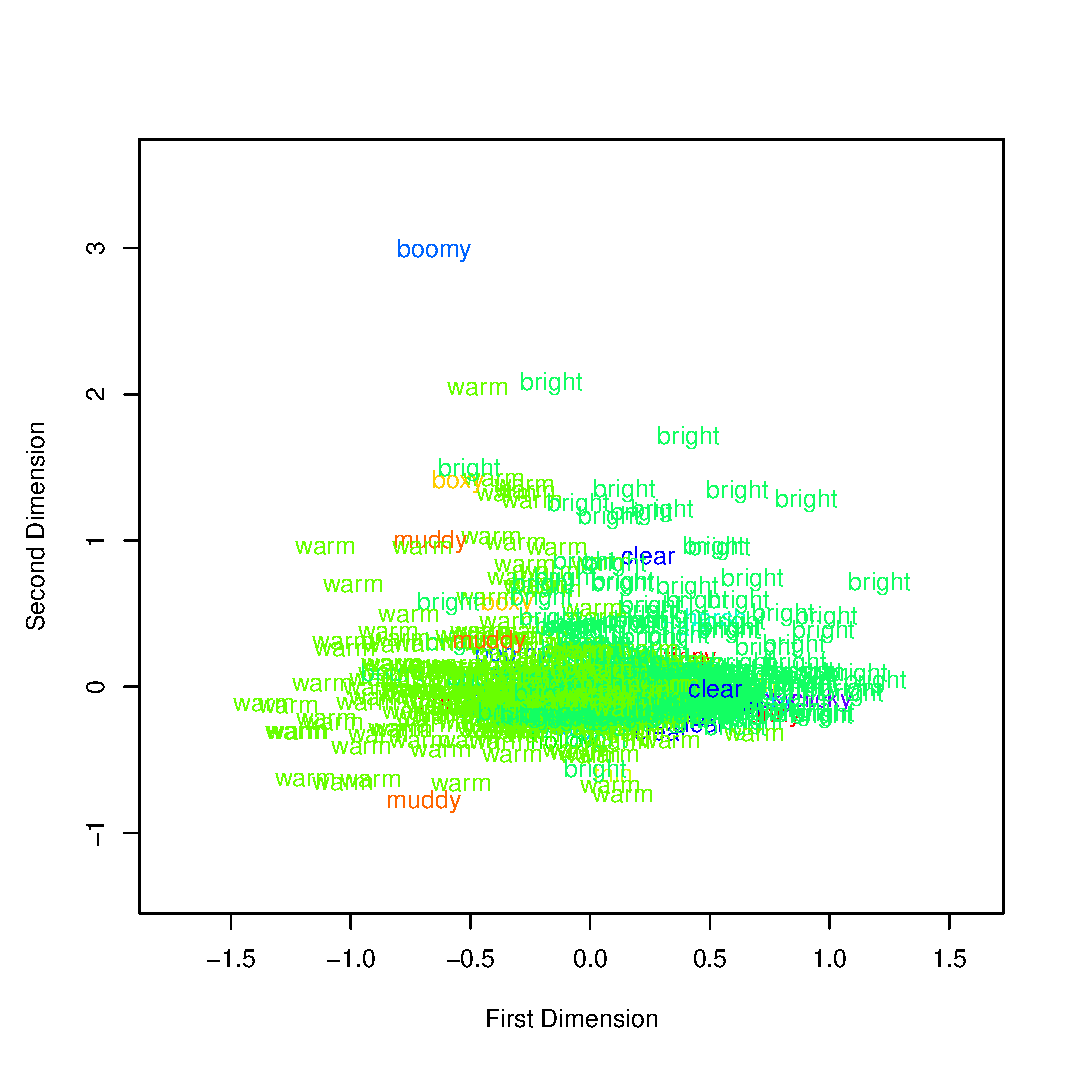
\includegraphics[width=0.45\textwidth]{chapter4/Images/EqualiserDifferenceMDS.eps}
			\label{fig:EqualiserDifferenceMDS}
		}
		\qquad
		\subfloat[Descriptor Centroids]
		{
			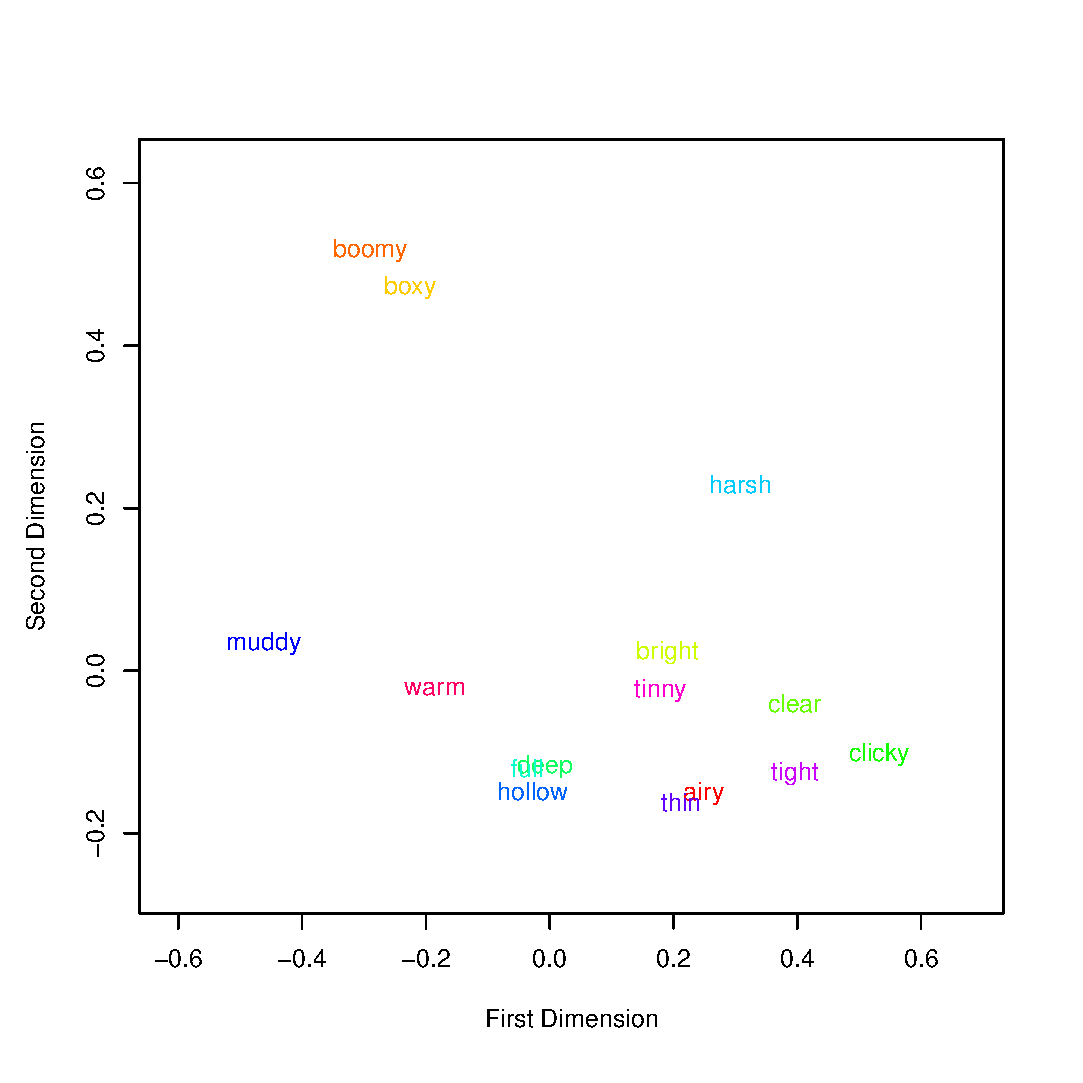
\includegraphics[width=0.45\textwidth]{chapter4/Images/EqualiserDifferenceCentroidsMDS.eps}
			\label{fig:EqualiserDifferenceCentroidsMDS}
		}
		\caption{Timbre Space for the Feature Differences form the Equaliser.}
		\label{fig:EqualiserDifferenceMDSs}
	\end{figure}

	\begin{table}[h!]
		\centering
		\begin{tabular}{|c|c|c|}
			\hline
			\bf{Feature} & \bf{Correlation} & \bf{p-value} \\
			\hline
			\hline
			Peak Tristimulus 2 & -0.890277830827284 & 3.45856612780454e-303 \\
			\hline
			Noisiness & -0.88597695501459 & 2.88937242814623e-296 \\
			\hline
			Harmonic Tristimulus 2 & -0.885741541888379 & 6.78585002438152e-296 \\
			\hline
			Harmonic Tristimulus 1 & -0.853307554457384 & 2.14548358937076e-251 \\
			\hline
			Peak Tristimulus 1 & -0.849822882281384 & 2.91473980458935e-247 \\
			\hline
			Fundamental & -0.816606742868406 & 1.74533328383416e-212 \\
			\hline
		\end{tabular}
		\caption{Significant Features for Dimension 1 of the Timbre Spaces Shown in Figure 
			 \ref{fig:EqualiserDifferenceMDSs}.}
		\label{tab:EqualiserDifferenceFeatures}
	\end{table}

	\begin{table}[h!]
		\centering
		\begin{tabular}{|c|c|c|}
			\hline
			\bf{Feature} & \bf{Correlation} & \bf{p-value} \\
			\hline
			\hline
			Irregularity K & 0.966464851638525 & 0 \\
			\hline
			Spectral Skewness & 0.942017154084719 & 0 \\
			\hline
			Spectral Kurtosis & 0.926960543352505 & 0 \\
			\hline
			Peak Irregularity K & 0.923930211100233 & 0 \\
			\hline
			Harmonic Irregularity K & 0.87430845721457 & 0 \\
			\hline
			Harmonic Spectral Kurtosis & 0.864277303727579 & 0 \\
			\hline
			Bark Coefficient 8 & 0.82502660118746 & 0 \\
			\hline
			Bark Coefficient 9 & 0.814424386595492 & 0 \\
			\hline
			Bark Coefficient 7 & 0.803206404903236 & 0 \\
			\hline
		\end{tabular}
		\caption{Significant Features for Dimension 2 of the Timbre Spaces Shown in Figure 
			 \ref{fig:EqualiserDifferenceMDSs}.}
		\label{tab:EqualiserDifferenceFeatures}
	\end{table}
